% !TeX program = pdflatex
%==============================================================================
%  BẢN DỊCH TIẾNG VIỆT
%  "Interpretable Bilingual Multimodal Large Language Model for Diverse
%   Biomedical Tasks" (MedRegA) -- ICLR 2025
%  Bản dịch phục vụ seminar môn Học sâu.
%  Quy ước: các hình của bài báo gốc được để dưới dạng PLACEHOLDER, chèn ảnh sau.
%==============================================================================
\documentclass[12pt,a4paper,oneside]{extarticle}
\usepackage[utf8]{inputenc}      % nhập liệu UTF-8 (pdfLaTeX)
\usepackage[T5]{fontenc}         % mã font T5 -- hỗ trợ tiếng Việt
\usepackage{mathptmx}            % font chữ kiểu Times (tương thích pdfLaTeX)

\usepackage{tikz}
\usetikzlibrary{positioning,arrows.meta}

\usepackage{float}
\usepackage{adjustbox}

\fontsize{13pt}{15pt}\selectfont

\usepackage[vietnamese]{babel}
% Dùng pdfLaTeX: chữ kiểu Times qua mathptmx (ở trên), tiếng Việt qua T5 + utf8.

%---- Lề trang & line spacing -----------------------------------------------
\usepackage[a4paper, top=2.5cm, bottom=2.5cm, left=3cm, right=2cm]{geometry}
\usepackage{setspace}
\onehalfspacing                            % cách dòng 1.5 (chuẩn báo cáo)

%---- Toán học --------------------------------------------------------------
\usepackage{amsmath, amssymb, amsfonts, amsthm}
\usepackage{bm}
\usepackage{mathtools}

%---- Đồ họa, bảng, code ----------------------------------------------------
\usepackage{graphicx}
\usepackage{caption}
\usepackage{subcaption}
\usepackage{array, tabularx, booktabs, multirow, makecell}
\usepackage{xcolor}
\newcolumntype{Y}{>{\raggedright\arraybackslash}X}
\newcolumntype{C}[1]{>{\centering\arraybackslash}m{#1}}

%---- Hyperlink & mục lục ---------------------------------------------------
\usepackage[colorlinks=true, linkcolor=black, citecolor=blue,
            urlcolor=blue, bookmarks=true]{hyperref}
\usepackage{tocloft}
\renewcommand{\cfttoctitlefont}{\Large\bfseries}

%---- Header / footer -------------------------------------------------------
\usepackage{fancyhdr}
\pagestyle{fancy}
\fancyhf{}
\fancyfoot[C]{\thepage}
\renewcommand{\headrulewidth}{0pt}

%---- Tiêu đề mục (override) ------------------------------------------------
\usepackage{titlesec}
\titleformat{\section}{\Large\bfseries}{\thesection.}{0.5em}{}
\titleformat{\subsection}{\large\bfseries}{\thesubsection.}{0.5em}{}
\titleformat{\subsubsection}{\normalsize\bfseries}{\thesubsubsection.}{0.5em}{}
\titlespacing*{\section}{0pt}{14pt}{8pt}
\titlespacing*{\subsection}{0pt}{12pt}{6pt}

%==============================================================================
\begin{document}

%---- TRANG BÌA -------------------------------------------------------------
\begin{titlepage}
\begin{center}

{\large\bfseries ĐẠI HỌC QUỐC GIA TP HỒ CHÍ MINH}\\[2pt]
{\large\bfseries TRƯỜNG ĐẠI HỌC KHOA HỌC TỰ NHIÊN}\\[2pt]
{\large\bfseries KHOA CÔNG NGHỆ THÔNG TIN}\\[0.5cm]

% Logo trường (tùy chọn): bỏ comment dòng dưới nếu có file logo.
% \includegraphics[width=0.3\textwidth]{figures/hcmus-logo.png}\\[0.5cm]
\vspace{0.5cm}

{\large BÁO CÁO MÔN HỌC SÂU}\\[6pt]

{\large\bfseries Bản dịch bài báo:}\\[8pt]
{\LARGE\bfseries Mô Hình Ngôn Ngữ Lớn Đa Phương Thức Song Ngữ Có Thể Diễn Giải cho Các Tác Vụ Y Sinh Đa Dạng}\\[1.2cm]
{\large\bfseries Bài báo gốc:}\\[2pt]
{\large\itshape ``Interpretable Bilingual Multimodal Large Language Model\\
for Diverse Biomedical Tasks''}\\[2pt]
{\large Lehan Wang, Haonan Wang, Honglong Yang, Jiaji Mao,\\
Zehong Yang, Jun Shen, and Xiaomeng Li}\\[2pt]
{\normalsize The Thirteenth International Conference on Learning Representations\\
(ICLR 2025)}\\[1cm]

\begin{flushleft}
\hspace{2cm}\begin{tabular}{ll}
\textbf{GIÁO VIÊN HƯỚNG DẪN:}   & TS. Nguyễn Tiến Huy \\
                                & TS. Lê Thanh Tùng\\[8pt]

\textbf{HỌC VIÊN THỰC HIỆN:}  & 25C15029 -- Lê Thị Tường Vy\\
                              & 25C15008 -- Phạm Ngọc Hiếu\\
                              & 25C15011 -- Nguyễn Huy Hoàng\\
                              & 25C11050 -- Nguyễn Đình Lộc\\
                              & 25C15003 -- Ngô Trương Minh Đạt\\
\end{tabular}
\end{flushleft}

\vfill
{\bfseries TPHCM -- 06/2026}

\end{center}
\end{titlepage}

%---- MỤC LỤC ---------------------------------------------------------------
\renewcommand{\contentsname}{MỤC LỤC}
\pagenumbering{roman}
\tableofcontents
\newpage

\pagenumbering{arabic}
\setcounter{page}{1}

% ============ TÓM TẮT ============
\section*{Tóm tắt}
\addcontentsline{toc}{section}{Tóm tắt}

Nhiều Mô hình Ngôn ngữ Lớn Đa phương thức (Multimodal Large Language Models -- MLLM)
trong y khoa đã được phát triển để giải quyết các tác vụ liên quan đến hình ảnh kèm
chỉ dẫn dạng văn bản trên nhiều phương thức (modality) y khoa khác nhau và đạt được
những kết quả ấn tượng. Tuy nhiên, hầu hết các mô hình tổng quát (generalist) trong y
khoa hiện nay đều \emph{không nhận biết vùng} (region-agnostic): chúng xử lý toàn bộ ảnh
như một biểu diễn tổng thể, nhưng lại khó xác định chính xác chúng
đang tập trung vào vùng nào khi sinh ra một câu mô tả. Để mô phỏng hành vi của bác sĩ --
những người thường bắt đầu bằng việc xem toàn bộ ảnh trước khi tập trung vào các vùng cụ
thể để đánh giá kỹ lưỡng -- nhóm tác giả hướng đến việc nâng cao khả năng của MLLM y khoa
trong việc hiểu các vùng giải phẫu bên trong toàn bộ ảnh chụp y khoa.

Để đạt được điều đó, nhóm tác giả trước hết \emph{định nghĩa các tác vụ lấy vùng làm trung
tâm} (Region-Centric tasks) và xây dựng một bộ dữ liệu quy mô lớn, \textbf{MedRegInstruct},
nhằm tích hợp thông tin vùng vào quá trình huấn luyện. Kết hợp bộ dữ liệu thu thập được với
các kho ngữ liệu đa phương thức y khoa khác, nhóm tác giả đề xuất một MLLM y khoa \emph{có
nhận biết vùng} (Region-Aware) tên là \textbf{MedRegA} -- hệ thống AI y khoa tổng quát song
ngữ đầu tiên có khả năng xử lý đồng thời các tác vụ thị giác--ngôn ngữ ở cả \emph{cấp độ ảnh}
và \emph{cấp độ vùng} trên một phạm vi rộng các phương thức. MedRegA không chỉ hỗ trợ ba tác
vụ lấy vùng làm trung tâm, mà còn đạt hiệu năng tốt nhất ở các tác vụ trả lời câu hỏi dựa trên
hình ảnh (VQA), sinh báo cáo và phân loại ảnh y khoa trên 8 phương thức, thể hiện tính đa năng
đáng kể. Các thí nghiệm cho thấy mô hình không chỉ đạt hiệu năng mạnh mẽ trên nhiều tác vụ
thị giác--ngôn ngữ y khoa trong bối cảnh song ngữ, mà còn có thể nhận diện và phát hiện các
cấu trúc trong ảnh quét y khoa đa phương thức, qua đó tăng cường tính diễn giải
(interpretability) và khả năng tương tác với người dùng của MLLM y khoa. Trang dự án:
\url{https://medrega.github.io}.

\begin{figure}[H]
\centering
\includegraphics[width=0.92\textwidth]{figures/fig1.png}
\caption{Tổng quan MedRegA -- mô hình tổng quát song ngữ có thể diễn giải cho nhiều tác vụ y
sinh, nổi bật ở khả năng khai thác thông tin vùng. MedRegA có thể tri nhận 8 phương thức bao
phủ gần như toàn bộ các bộ phận cơ thể. (Hình~1 của bài báo gốc.)}
\end{figure}

\newpage

% ============ 1. GIỚI THIỆU ============
\section{Giới thiệu}

Trong những năm gần đây, các Mô hình Ngôn ngữ Lớn Đa phương thức (MLLM) đã có những bước
tiến nhanh chóng và tỏ ra nhiều hứa hẹn khi được áp dụng vào lĩnh vực chăm sóc sức khỏe.
Bằng cách tích hợp phương thức thị giác và văn bản, MLLM có thể đáp ứng nhiều nhu cầu y khoa
đa dạng như tư vấn bệnh nhân, sinh báo cáo y khoa và chẩn đoán bệnh. Một số mô hình Trí tuệ
Nhân tạo (AI) trong y khoa đã được đề xuất để xử lý các tác vụ khác nhau liên quan đến ảnh kèm
chỉ dẫn văn bản trên nhiều phương thức và đạt kết quả ấn tượng.

Tuy nhiên, phần lớn các mô hình tổng quát y khoa hiện nay đều \emph{không nhận biết vùng}:
chúng được thiết kế để coi toàn bộ ảnh như một biểu diễn tổng thể, nhưng lại khó khăn trong
việc phát hiện hoặc suy luận về các vùng cụ thể bên trong một ảnh quét y khoa. Sự thiếu hụt
nhận thức không gian này thường dẫn đến những mô tả không chính xác, làm giảm chất lượng báo
cáo được sinh ra. Như minh họa ở Hình~2(a), các mô hình không nhận biết vùng (ví dụ MedDr) đã
nhận nhầm vùng tổn thương ở phần \emph{bên trái} của não, trong khi sự thật (ground truth) lại
nằm ở phần \emph{bên phải}. Việc định vị sai này khiến MedDr phân loại tổn thương thành phù nề
xung quanh (surrounding edema) thay vì u thần kinh đệm (glioma) như nhận định của bác sĩ chẩn
đoán hình ảnh. Hệ quả là các bác sĩ lâm sàng khó kiểm chứng, tin tưởng hay chỉnh sửa báo cáo
được sinh ra, làm cản trở tính diễn giải và khả năng ứng dụng lâm sàng của mô hình.

Thách thức cốt lõi nảy sinh do các phương pháp trước đây \emph{không được huấn luyện trên các
tác vụ lấy vùng làm trung tâm}. Cụ thể, báo cáo y khoa thường gồm nhiều mô tả về nhiều vùng
khác nhau, khiến ta không rõ mô hình đang đề cập đến vùng nào cho mỗi câu được sinh ra. Sự mơ
hồ này làm giảm độ tin cậy và không phù hợp với quy trình lâm sàng. Bác sĩ chẩn đoán hình ảnh
thường bắt đầu bằng việc xem toàn bộ ảnh, rồi mới tập trung vào các vùng cụ thể để đảm bảo
đánh giá kỹ lưỡng. Lấy cảm hứng từ quy trình này, nhóm tác giả hướng đến việc tích hợp thông
tin lấy vùng làm trung tâm vào MLLM y khoa, phản ánh đúng quy trình làm việc của bác sĩ. Cách
tiếp cận này rất quan trọng vì nó đảm bảo mô hình tập trung đúng vào vùng đang được mô tả, dù
là vùng bình thường, bất thường, chưa chắc chắn, hay ở bất kỳ trạng thái nào.

\begin{figure}[H]
\centering
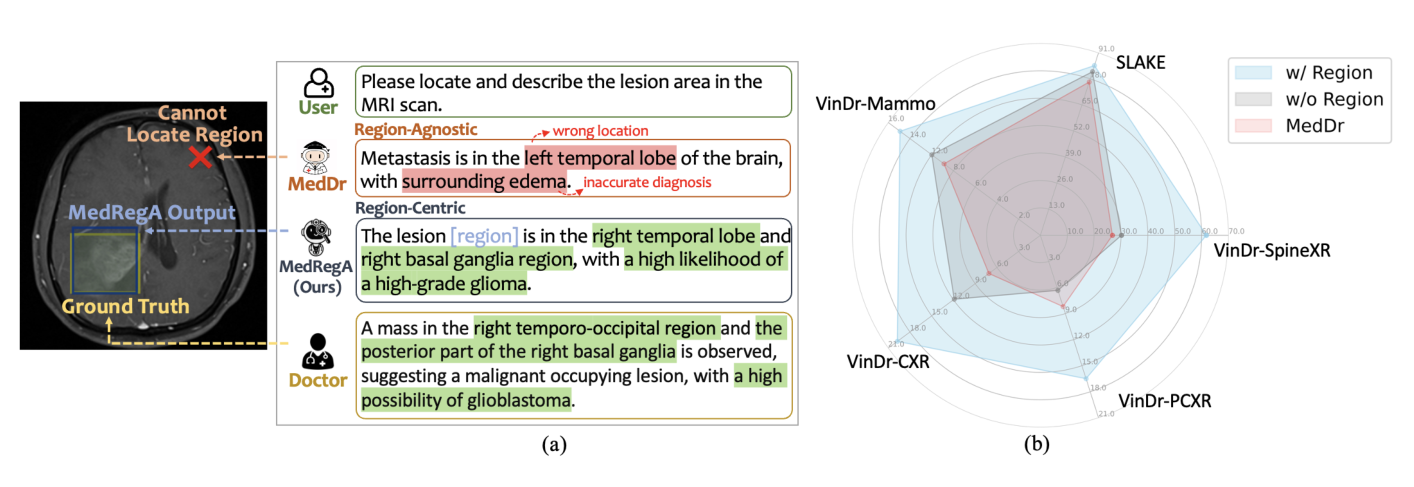
\includegraphics[width=0.95\textwidth]{figures/fig2.png}
\caption{Tầm quan trọng của khả năng lấy vùng làm trung tâm. (a) So sánh giữa mô hình không nhận
biết vùng (MedDr) và mô hình lấy vùng làm trung tâm (MedRegA) khi phân tích vùng tổn thương trong
ảnh quét y khoa. (b) So sánh hiệu năng khi nhắc (prompt) mô hình có và không có thông tin vùng
trên năm benchmark của tác vụ VQA và phân loại. (Hình~2 của bài báo gốc.)}
\end{figure}

Để khắc phục các hạn chế nêu trên, nhóm tác giả trước hết giới thiệu \textbf{ba tác vụ lấy
vùng làm trung tâm}:
\begin{enumerate}
  \item \textbf{Nhận dạng Vùng--sang--Văn bản} (Region-to-Text Identification): nhận diện cấu
  trúc, cơ quan hoặc bất thường nằm trong một hộp giới hạn (bounding box) cho trước được đưa
  vào làm đầu vào.
  \item \textbf{Phát hiện Văn bản--sang--Vùng} (Text-to-Region Detection): định vị chính xác
  vị trí của các cấu trúc hoặc bất thường được mô tả trong chỉ dẫn bằng cách sinh ra các hộp
  giới hạn.
  \item \textbf{Sinh Báo cáo có Định vị} (Grounded Report Generation): sinh báo cáo chi tiết
  kèm theo hộp giới hạn tương ứng cho các cấu trúc giải phẫu liên quan trong ảnh y khoa.
\end{enumerate}

Để giúp MLLM thực hiện được ba tác vụ này, nhóm tác giả xây dựng một bộ dữ liệu quy mô lớn
\textbf{MedRegInstruct} bao gồm tất cả các tác vụ trên. Nhóm thu thập dữ liệu lâm sàng thực tế
từ Bệnh viện Tưởng niệm Tôn Trung Sơn (Sun Yat-Sen Memorial Hospital), gồm khoảng 25.000 cặp
ảnh quét--báo cáo tiếng Trung thuộc các phương thức X-quang, CT và MRI từ 15.000 bệnh nhân.
Sau đó, nhóm đề xuất một hệ thống gán nhãn tự động để biên soạn các báo cáo có định vị, giúp
giảm chi phí gán nhãn thủ công chi tiết cho từng cơ quan trong mỗi ảnh quét y khoa.

Kết hợp bộ dữ liệu thu thập được MedRegInstruct với các kho ngữ liệu đa phương thức y khoa khác
để huấn luyện, nhóm tác giả đề xuất một MLLM y khoa có nhận biết vùng, \textbf{MedRegA} -- hệ
thống AI y khoa tổng quát song ngữ đầu tiên xử lý đồng thời các tác vụ thị giác--ngôn ngữ ở cấp
độ ảnh và cấp độ vùng trên một phạm vi rộng các phương thức như chẩn đoán hình ảnh (radiology),
giải phẫu bệnh (pathology), da liễu (dermatology) và nhãn khoa (ophthalmology); xem Hình~1. Các
thí nghiệm trình bày ở Hình~2(b) cho thấy MedRegA có thể xuất ra chính xác hộp giới hạn của vùng
cụ thể đang được tập trung, trong khi các MLLM y khoa tốt nhất hiện có không làm được. Điều này
giúp mô hình mô tả đúng tình trạng của các vùng nhất định (Hình~2a) và còn nâng cao các tác vụ
hạ nguồn khác như trả lời câu hỏi dựa trên hình ảnh và chẩn đoán (Hình~2b). Tóm lại, MedRegA
vượt MedDr lần lượt 3,91\% và 8,03\% (BLEU-1) trên MIMIC-CXR và IU-Xray ở tác vụ sinh báo cáo
tiếng Anh, cùng mức cải thiện thêm 27,34\% khi sinh báo cáo tiếng Trung. Bên cạnh đó, MedRegA
không chỉ hỗ trợ ba tác vụ lấy vùng làm trung tâm mà còn đạt hiệu năng tốt nhất ở VQA, sinh báo
cáo và phân loại ảnh y khoa trên 8 phương thức, thể hiện tính đa năng đáng kể.

Tóm lại, các \textbf{đóng góp} của bài báo gồm:
\begin{enumerate}
  \item Thiết lập các \emph{tác vụ lấy vùng làm trung tâm} với bộ dữ liệu quy mô lớn
  MedRegInstruct, trong đó mỗi mẫu được ghép cặp với tọa độ của các cấu trúc cơ thể hoặc tổn
  thương. Điều này mở rộng chức năng của mô hình để tri nhận các vùng bên trong ảnh quét y khoa,
  khuyến khích mô hình tập trung vào những vùng quan trọng và cải thiện tính diễn giải. Để
  đánh giá năng lực vùng của MLLM y khoa, nhóm đề xuất một \emph{khung đánh giá căn chỉnh theo
  vùng} (Region-Aligned evaluation) nhằm đo lường chất lượng và mức độ căn chỉnh giữa văn bản
  và vùng được sinh ra.
  \item Dựa trên bộ dữ liệu đề xuất, nhóm phát triển MLLM y khoa có nhận biết vùng MedRegA như
  một hệ thống AI y khoa tổng quát song ngữ, thực hiện cả tác vụ cấp độ ảnh lẫn cấp độ vùng. Ở
  giai đoạn suy luận, nhóm giới thiệu \emph{Chuỗi Suy luận theo Vùng} (Regional Chain-of-Thought
  -- Regional CoT) để tăng cường hiệu năng nhờ tri thức không gian của mô hình.
  \item Nhóm đánh giá mô hình trên các tác vụ y khoa toàn diện gồm VQA, sinh báo cáo, phân loại
  ảnh, nhận dạng vùng, phát hiện vùng và sinh báo cáo có định vị. MedRegA vượt các phương pháp
  SOTA với khoảng cách lớn trên cả tác vụ thị giác--ngôn ngữ truyền thống lẫn tác vụ lấy vùng
  làm trung tâm.
\end{enumerate}

% ============ 2. NGHIÊN CỨU LIÊN QUAN ============
\section{Nghiên cứu liên quan}

\subsection{Bộ dữ liệu Thị giác--Ngôn ngữ cho Y khoa}

Trong quá trình phát triển MLLM, có một nhu cầu lớn về các bộ dữ liệu ảnh--văn bản dùng làm
nguồn dữ liệu tiền huấn luyện, bởi các bộ dữ liệu này đóng vai trò then chốt đối với hiệu năng
mô hình. Các bộ dữ liệu thị giác--ngôn ngữ phổ biến nhất trong y khoa bao gồm những bộ dành cho
tác vụ trả lời câu hỏi dựa trên hình ảnh (VQA) và sinh báo cáo y khoa (MRG). Tuy nhiên, các bộ
dữ liệu này thiếu chú thích vùng tương ứng với văn bản, cản trở MLLM hiểu sâu hơn về thông tin
cấu trúc bên trong ảnh quét y khoa. Một số công trình đã cố gắng thu hẹp khoảng cách này bằng
cách tích hợp định vị vùng vào hội thoại đa phương thức, nhưng lại hạn chế về khả năng tiếp cận
các mô tả được viết thủ công từ tình huống lâm sàng thực tế. Mặc dù một số công trình khác đã
xây dựng báo cáo theo vùng ghép cặp với mặt nạ bất thường (anomaly mask) từ dữ liệu lâm sàng,
chúng chỉ tập trung lần lượt vào CT lồng ngực và MRI não, vẫn để trống các cấu trúc cơ thể khác
như đại tràng, gan và tụy. Do đó, các bộ dữ liệu hiện có chưa đáp ứng yêu cầu phát triển một
MLLM tổng quát trong y tế, đặc biệt là khả năng hiểu thông tin vùng và tiếp nhận đầu vào đa
phương thức đa dạng từ nhiều hệ thống y khoa. Điều này đặt ra thách thức đáng kể trong việc
tạo ra một mô hình có thể hỗ trợ hiệu quả cho bác sĩ lâm sàng trên nhiều chuyên khoa khác nhau.

\subsection{Mô hình Ngôn ngữ Lớn Đa phương thức trong Y khoa}

Tiến bộ nhanh chóng của MLLM đã thúc đẩy việc tích hợp chúng vào lĩnh vực y khoa nhằm nâng cao
quá trình chẩn đoán, nghiên cứu y học và chăm sóc bệnh nhân. Việc phát triển các mô hình y khoa
quy mô lớn đi theo xu hướng mở rộng dần phạm vi ứng dụng. Một số trợ lý AI được thiết kế chuyên
biệt cho một phương thức duy nhất. Nhờ nguồn dữ liệu công khai dồi dào cho ảnh X-quang ngực
(CXR), nhiều công trình đã hỗ trợ MLLM hiểu được ảnh CXR. Riêng với giải phẫu bệnh, có công
trình đã biên soạn một bộ dữ liệu ảnh bệnh học quy mô lớn và trình bày một trợ lý AI bệnh học.
Vì số lượng tham số lớn của MLLM cho phép chúng lưu trữ tri thức trên nhiều phương thức, nhiều
công trình đã mở rộng phạm vi bao phủ của ảnh y khoa để triển khai các MLLM y khoa tổng quát và
khả dụng hơn. Tuy nhiên, do thiếu khả năng nhận diện và phát hiện cấu trúc giải phẫu bên trong
ảnh quét, các mô hình trước đây vẫn gặp khó khăn trong việc đưa ra mô tả chi tiết như chuyên gia
về các cấu trúc hoặc tổn thương cụ thể, làm hạn chế đáng kể độ tin cậy và tính diễn giải.

\subsection{Mô hình Ngôn ngữ Lớn Đa phương thức có Khả năng Vùng}

Nâng cao khả năng vùng để tri nhận các đối tượng cụ thể và gắn (ground) các phản hồi với những
vùng liên quan là yếu tố then chốt giúp ích cho hiểu biết thị giác, khiến đây trở thành một mục
tiêu phổ biến khi huấn luyện MLLM cho ảnh tự nhiên. Tuy nhiên, việc giúp MLLM phát hiện và định
vị các cấu trúc chi tiết trong ảnh y khoa vẫn còn ít được khám phá. Nghiên cứu hiện tại chủ yếu
tập trung vào một tập hạn chế các tác vụ liên quan đến vùng, chỉ với một vài phương thức. Chẳng
hạn, một số mô hình có khả năng phát hiện cấu trúc đơn lẻ dựa trên prompt cho trước, nhưng không
phác họa được mô tả chi tiết cho từng vùng như một bác sĩ lâm sàng có thể làm. Một công trình
khác đã giới thiệu tác vụ sinh báo cáo có định vị và phát triển một MLLM sinh mô tả cho tất cả
phát hiện trong ảnh y khoa kèm vị trí tương ứng, nhưng mô hình lại bị giới hạn chỉ nhận đầu vào
là ảnh X-quang ngực. Trên cơ sở các hạn chế này, nhóm tác giả hướng đến việc tích hợp đầy đủ
chức năng nhận diện, phát hiện và mô tả vùng cho một phạm vi rộng các phương thức vào mô hình
được đề xuất.

% ============ 3. XÂY DỰNG BỘ DỮ LIỆU ============
\section{Xây dựng Bộ dữ liệu Lấy vùng làm Trung tâm}

Trong phần này, nhóm tác giả giới thiệu bộ dữ liệu \textbf{MedRegInstruct}, gồm hai bộ con:
(1) \emph{Bộ dữ liệu Vùng--Văn bản} (Region-Text Dataset) chứa 550.000 bộ ba gồm ảnh, cặp
câu hỏi--câu trả lời, và vùng tương ứng; (2) \emph{Bộ dữ liệu Báo cáo có Định vị}
(Region-Grounded Dataset) gồm 240.000 mẫu, trong đó mỗi ảnh đi kèm một báo cáo được chú thích
theo vùng và mô tả chi tiết cho từng vùng. So với các bộ dữ liệu thị giác--ngôn ngữ y khoa
trước đây, bộ dữ liệu này không chỉ nhấn mạnh thêm vào việc bồi dưỡng khả năng vùng của MLLM y
khoa, mà còn tăng đáng kể tính đa dạng nhờ tích hợp một phạm vi rộng hơn các cấu trúc giải phẫu
và bối cảnh song ngữ cho việc sinh báo cáo. (Chi tiết phân bố dữ liệu xem Phụ lục~A.1 của bài
báo gốc.)

\subsection{Bộ dữ liệu Vùng--Văn bản}

Bộ dữ liệu Vùng--Văn bản được tạo ra từ SA-Med2D-20M -- một bộ dữ liệu phân đoạn quy mô lớn
chứa ảnh y khoa 2D của gần như toàn bộ các bộ phận cơ thể. Nhóm lọc khoảng 285.000 ảnh từ bộ
dữ liệu gốc để duy trì tính đa dạng của các cấu trúc giải phẫu và tổn thương bất thường. Các
mặt nạ phân đoạn đã được gán nhãn ban đầu được chuyển thành hộp giới hạn để biểu diễn vùng cần
làm nổi bật. Các cặp ảnh--vùng được hình thành theo hai dạng: (1) \emph{Vùng--sang--Văn bản}:
mô hình xuất ra thông tin của vùng được làm nổi bật khi cho trước hộp giới hạn; (2)
\emph{Văn bản--sang--Vùng}: mô hình định vị các vùng cụ thể bằng cách sinh ra hộp giới hạn. Để
thu được các cặp câu hỏi--câu trả lời, nhóm điền tên vùng và tọa độ vào các mẫu (template) định
nghĩa sẵn. Về mặt thống kê, bộ dữ liệu Vùng--Văn bản chứa 550.000 mục, với khoảng một nửa dành
cho Vùng--sang--Văn bản và nửa còn lại cho Văn bản--sang--Vùng.

\subsection{Bộ dữ liệu Báo cáo có Định vị}

Bộ dữ liệu báo cáo có định vị được lấy từ hai nguồn: bộ dữ liệu MIMIC-CXR và dữ liệu lâm sàng
nội bộ gồm 25.000 ảnh quét X-quang, MRI và CT từ 15.000 bệnh nhân. Dữ liệu nội bộ bao phủ nhiều
vùng gồm não, bụng, ngực, cột sống và khung chậu. Quy trình xử lý dữ liệu tự động để biên soạn
báo cáo có định vị gồm ba bước: \emph{Xây dựng cặp Ảnh--Báo cáo}, \emph{Tinh chỉnh Báo cáo} và
\emph{Phát hiện Cấu trúc}.

\begin{figure}[H]
\centering
\includegraphics[width=0.95\textwidth]{figures/fig3.png}
\caption{Quy trình xây dựng dữ liệu cho Bộ dữ liệu Báo cáo có Định vị. Quy trình xử lý tự động
gồm ba bước: Xây dựng cặp Ảnh--Báo cáo, Tinh chỉnh Báo cáo và Phát hiện Cấu trúc. (Hình~3 của
bài báo gốc.)}
\end{figure}

\noindent\textbf{Xây dựng cặp Ảnh--Báo cáo.} Với bộ dữ liệu MIMIC-CXR, nhóm theo các công trình
trước, sử dụng cả ảnh chụp thẳng (frontal) và chụp nghiêng (lateral), đồng thời đưa cả phần phát
hiện (findings) và phần ấn tượng/kết luận (impressions) vào báo cáo. Với bộ dữ liệu nội bộ, nhóm
trích các lát cắt trung tâm từ mỗi ảnh quét 3D để tạo đầu vào 2D -- thường cung cấp góc nhìn đại
diện nhất cho các cấu trúc giải phẫu. Tổng cộng, nhóm xây dựng 95.000 cặp ảnh--báo cáo từ dữ liệu
lâm sàng thu thập được, có thể dùng để kích thích khả năng song ngữ của MLLM bằng cách tăng cường
sinh báo cáo có cấu trúc bằng tiếng Trung.

\noindent\textbf{Tinh chỉnh Báo cáo.} Mục tiêu là phân rã dữ liệu báo cáo thô thành các mô tả
chi tiết cho từng cơ quan được đề cập trong ảnh quét y khoa. Nhóm nhận thấy mô hình mã nguồn mở
InternLM thể hiện khả năng hiểu văn bản ấn tượng đối với báo cáo y khoa tiếng Trung. Để tận dụng
tốt khả năng trích xuất thông tin của LLM, nhóm trước hết áp dụng một chiến lược dựa trên luật
(rule-based) để tóm tắt sơ bộ tất cả các cơ quan được nhắc đến trong báo cáo. Sau đó, nhóm dùng
InternLM để phân tách mỗi báo cáo thành các mô tả chi tiết với danh sách cơ quan được đưa vào
làm prompt.

\noindent\textbf{Phát hiện Cấu trúc.} Với bộ MIMIC-CXR -- đã được Chest ImaGenome gán nhãn tọa
độ hộp giới hạn cho 29 vị trí giải phẫu -- nhóm chọn 12 vị trí chuẩn hóa ở vùng ngực. Sau đó,
nhóm kết hợp các hộp giới hạn đã chọn với mô tả tương ứng trong các báo cáo đã phân tách để tạo
thành báo cáo có định vị theo vùng cho ảnh X-quang ngực. Tổng cộng, 220.000 báo cáo có định vị
được xây dựng từ MIMIC-CXR. Với bộ dữ liệu nội bộ, một số ảnh quét được gán nhãn thủ công vùng
tổn thương như u não, ung thư phổi và các bất thường khác. Tuy nhiên, vẫn cần nhãn vùng cho các
cấu trúc giải phẫu. Để tự động định vị các cơ quan quan sát được trong ảnh quét, nhóm trước hết
tinh chỉnh (finetune) một MLLM dựa trên bộ dữ liệu Vùng--Văn bản, vốn chứa ảnh quét cùng phương
thức và cơ quan với dữ liệu thu thập. Sau đó, nhóm đưa các ảnh thu thập vào MLLM đã tinh chỉnh,
kèm prompt là các cơ quan có trong báo cáo, để thu được các hộp giới hạn tương ứng. Cuối cùng,
nhóm khớp tọa độ bất thường đã chú thích với mô tả phần tổn thương, và khớp các vùng cơ quan đã
phát hiện với phần tương ứng trong báo cáo đã phân tách.

\noindent\textbf{Kiểm định bởi con người.} Để đánh giá chất lượng phần dữ liệu được chú thích
tự động và đưa ra đánh giá định lượng, nhóm chọn ngẫu nhiên 50 mẫu và mời 2 chuyên gia tạo nhãn
thủ công để so sánh. Với bước Tinh chỉnh Báo cáo, độ chính xác ở mức câu (sentence-level) đạt
93,33\%. Với bước Phát hiện Cấu trúc, độ chính xác của hộp giới hạn được sinh ra đạt 72\% so với
chú thích của con người. Nhóm cũng tiến hành đánh giá trực quan và nhận thấy rằng mặc dù phần lớn
hộp giới hạn hơi lớn hơn so với vùng mục tiêu, chúng vẫn bao trùm được vùng đó. Điều này là đủ cho cách
tiếp cận của nhóm, vì nhóm chỉ cần định vị chứ không cần một hộp giới hạn thật khít và chính xác.

% ============ 4. PHƯƠNG PHÁP ============
\section{MLLM Y khoa có Nhận biết Vùng (MedRegA)}

MLLM y khoa có nhận biết vùng MedRegA đóng vai trò là một hệ thống AI y khoa song ngữ có thể
diễn giải, xử lý nhiều tác vụ thị giác--ngôn ngữ gồm VQA, sinh báo cáo và phân loại, với khả
năng vùng chuyên biệt cho các tác vụ lấy vùng làm trung tâm. Phần này lần lượt trình bày: cách
hình thức hóa các tác vụ lấy vùng làm trung tâm, quá trình huấn luyện mô hình, và chiến lược
sinh có hướng dẫn theo vùng nhằm cải thiện chất lượng suy luận.

\begin{figure}[H]
\centering
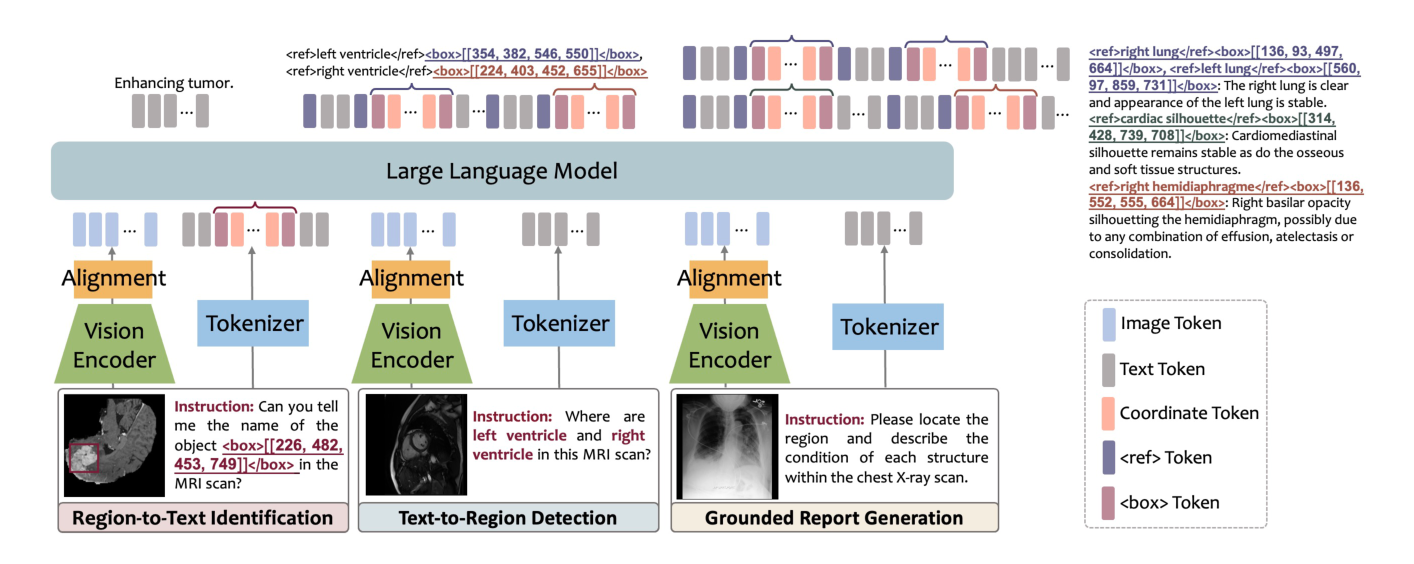
\includegraphics[width=0.95\textwidth]{figures/fig4.png}
\caption{Ví dụ minh họa việc thực hiện các tác vụ lấy vùng làm trung tâm với MedRegA. (Hình~4
của bài báo gốc.)}
\end{figure}

\noindent\textbf{Hình thức hóa Tác vụ Lấy vùng làm Trung tâm.} Nhóm định nghĩa các tác vụ lấy
vùng làm trung tâm theo ba góc độ: (1) \emph{Nhận dạng Vùng--sang--Văn bản}, mô hình xuất ra
tên của vùng được chỉ định; (2) \emph{Phát hiện Văn bản--sang--Vùng}, mô hình phát hiện vùng của
cơ quan hoặc bất thường cho trước; (3) \emph{Sinh Báo cáo có Định vị}, mô hình sinh báo cáo cho
ảnh quét y khoa, căn chỉnh mỗi mô tả với vùng tương ứng. Để mô hình mã hóa được thông tin vùng,
nhóm biểu diễn vùng dưới dạng hộp giới hạn $[x_1, y_1, x_2, y_2]$, trong đó $(x_1, y_1)$ là điểm
góc trên bên trái và $(x_2, y_2)$ là điểm góc dưới bên phải của hộp. Tất cả giá trị được chuẩn
hóa thành số nguyên trong khoảng $[0, 1000)$. Các hộp giới hạn này được chèn vào câu, bao quanh
bởi một cặp token đặc biệt, ví dụ \texttt{<box>[x1, y1, x2, y2]</box>}, trong khi đối tượng tương
quan được đánh dấu bằng \texttt{<ref></ref>}, như minh họa ở Hình~4.

\noindent\textbf{Huấn luyện Mô hình.} Để huấn luyện một MLLM y khoa tổng quát không chỉ giới hạn
ở việc hiểu vùng, nhóm xử lý và tích hợp nhiều bộ dữ liệu công khai cho các tác vụ khác nhau gồm
VQA, sinh báo cáo, phân loại cơ quan và chẩn đoán bệnh. Nhóm thiết kế các chỉ dẫn riêng cho từng
tác vụ để nhắc mô hình nhận diện và xử lý các mục tiêu khác nhau. Xét hiệu năng cạnh tranh của mô
hình mã nguồn mở InternVL~1.2, nhóm dùng nó làm nền tảng miền tổng quát để bắt đầu huấn luyện; mô
hình này gồm InternViT-6B làm bộ mã hóa thị giác (vision encoder) và Nous-Hermes-2-Yi-34B làm mô
hình ngôn ngữ. Quá trình huấn luyện chia làm hai bước: \emph{huấn luyện căn chỉnh} (alignment
training) và \emph{tinh chỉnh theo chỉ dẫn} (instruction tuning). Ở giai đoạn huấn luyện căn
chỉnh, nhóm đóng băng bộ mã hóa thị giác và mô hình ngôn ngữ, chỉ tinh chỉnh module căn chỉnh với
các bộ dữ liệu chú thích ảnh y khoa (image captioning). Ở giai đoạn tinh chỉnh theo chỉ dẫn, nhóm
dùng cả các bộ dữ liệu công khai lẫn bộ dữ liệu lấy vùng làm trung tâm MedRegInstruct để tối ưu
mô hình ngôn ngữ, giữ nguyên các thành phần còn lại. Hàm mất mát (loss) của mô hình ngôn ngữ được
dùng làm hàm mục tiêu. (Chi tiết huấn luyện xem Phụ lục~B của bài báo gốc.)

\noindent\textbf{Chuỗi Suy luận theo Vùng (Regional CoT).} Sau khi huấn luyện trên các tác vụ lấy
vùng làm trung tâm, mô hình đã có khả năng nhận dạng và phát hiện vùng, vốn có tiềm năng nâng cao
hiệu năng trên các tác vụ tổng quát khác. Như đã được chứng minh ở các công trình trước, việc văn
bản hóa thêm các hướng dẫn bổ sung như tọa độ không gian vào prompt sẽ giải phóng khả năng xử lý
thông tin đa phương thức của mô hình ngôn ngữ. Theo các nhận định này, nhóm tích hợp Regional CoT
vào quy trình sinh để khai thác tốt hơn các kỹ năng vùng, như minh họa ở Hình~5. Mô hình trước
hết phải phát hiện các vùng quan trọng trong ảnh đầu vào, sau đó thực hiện sinh với prompt là các
vùng đã phát hiện. Cách tiếp cận này khuyến khích mô hình chú ý nhiều hơn đến các cấu trúc bên
trong ảnh quét y khoa khi trả lời tư vấn bệnh nhân hoặc chẩn đoán bệnh.

\begin{figure}[H]
\centering
\includegraphics[width=0.98\textwidth]{figures/fig5.png}
\caption{So sánh quy trình suy luận--sinh truyền thống với quy trình có Regional CoT. (Hình~5
của bài báo gốc.)}
\end{figure}

% ============ 5. THỰC NGHIỆM ============
\section{Thực nghiệm}

\subsection{Hiệu năng trên các Tác vụ Y khoa Tổng quát}

Để đánh giá khả năng của MedRegA trên các tác vụ y khoa tổng quát -- gồm VQA, sinh báo cáo và
phân loại -- nhóm so sánh toàn diện mô hình với mô hình nền InternVL và các MLLM y khoa mã nguồn
mở trong miền tổng quát, bao gồm Med-Flamingo, LLaVA-Med, RadFM, MedDr và BiomedGPT, bằng cách
tái lập các checkpoint đã công bố của chúng với chỉ dẫn prompt chính thức. Bảng~\ref{tab:main}
trình bày so sánh hiệu năng tổng thể với kết quả trung bình trên mỗi tác vụ. Cần lưu ý rằng các
baseline hiện có không thể định vị các vùng được làm nổi bật trong ảnh quét và không thể cung
cấp đầu ra vùng hợp lệ, bộc lộ một hạn chế lớn trong việc phân biệt cấu trúc cơ thể và phát hiện
bất thường chi tiết.

\begin{table}[H]
\centering
\caption{So sánh hiệu năng trên các tác vụ y khoa tổng quát và các tác vụ lấy vùng làm trung
tâm. ``N/A'' nghĩa là điểm không được báo cáo; ``-'' nghĩa là mô hình không sinh được đầu ra hợp
lệ; ``\texttt{x}'' nghĩa là mô hình không xử lý được tác vụ tương ứng; ``*'' nghĩa là
mô hình được tinh chỉnh trên bộ dữ liệu đó. (Trích từ Bảng~1 của bài báo gốc.)}
\label{tab:main}
\small
\setlength{\tabcolsep}{4pt}
\begin{adjustbox}{max width=\textwidth}
\begin{tabular}{llccccccc}
\toprule
\textbf{Tác vụ} & \textbf{Chỉ số} & \textbf{Med-Flamingo} & \textbf{LLaVA-Med} & \textbf{RadFM}
 & \textbf{MedDr} & \textbf{BiomedGPT} & \textbf{InternVL} & \textbf{MedRegA} \\
\midrule
\multicolumn{9}{c}{\textit{Trả lời câu hỏi dựa trên hình ảnh (VQA)}}\\
\midrule
\multirow{5}{*}{\makecell[l]{VQA\\Tiếng Anh}}
 & BLEU-1     & 21.16 & 54.59* & 51.19 & 65.72 & N/A    & 63.51 & \textbf{67.65} \\
 & F1         & 22.28 & 54.81* & 51.36 & 66.87 & N/A    & 65.05 & \textbf{68.33} \\
 & Acc (Close)& 41.91 & 43.73* & 61.01 & 84.03 & 86.40* & 64.99 & 83.25 \\
 & Recall (Open)&12.03& 63.51* & 42.63 & 49.81 & 57.73* & 44.17 & 53.35 \\
 & BertScore  & 53.20 & 75.73* & 73.29 & 77.80 & N/A    & 35.47 & \textbf{84.67} \\
\midrule
\multirow{5}{*}{\makecell[l]{VQA\\Tiếng Trung}}
 & BLEU-1     & 10.28 & 22.17 & 11.30 & 37.76 & N/A & 39.73 & \textbf{60.89} \\
 & F1         & 11.44 & 22.32 & 11.63 & 39.86 & N/A & 40.95 & \textbf{62.66} \\
 & Accuracy   & 13.46 & 16.50 & 12.32 & 35.53 & N/A & 38.02 & \textbf{58.64} \\
 & Recall     & 16.85 & 23.23 & 14.43 & 38.77 & N/A & 40.20 & \textbf{62.01} \\
 & BertScore  & 59.10 & 28.24 & 65.75 & 87.55 & N/A & 87.58 & \textbf{91.63} \\
\midrule
\multicolumn{9}{c}{\textit{Sinh báo cáo}}\\
\midrule
\multirow{5}{*}{\makecell[l]{Báo cáo\\Tiếng Anh}}
 & BLEU-1    & 21.50 & 17.47 & 29.06 & 34.49 & N/A    & 13.12 & \textbf{40.46} \\
 & BLEU-4    & 2.63  & 0.28  & 4.30  & 10.02 & N/A    & 0.53  & \textbf{12.60} \\
 & METEOR    & 17.30 & 12.68 & 19.38 & 27.70 & 13.55* & 14.26 & \textbf{31.94} \\
 & ROUGE-L   & 13.79 & 8.54  & 13.74 & 24.61 & 26.45* & 10.56 & \textbf{27.57} \\
 & BertScore & 49.81 & 44.34 & 53.43 & 55.12 & N/A    & 49.26 & \textbf{62.54} \\
\midrule
\multirow{5}{*}{\makecell[l]{Báo cáo\\Tiếng Trung}}
 & BLEU-1    & 3.59 & 4.91 & 3.66 & 11.99 & N/A & 10.71 & \textbf{40.76} \\
 & BLEU-4    & -    & -    & 0.02 & 0.32  & N/A & 1.85  & \textbf{18.74} \\
 & METEOR    & 2.59 & 3.60 & 4.05 & 10.71 & N/A & 9.68  & \textbf{34.03} \\
 & ROUGE-L   & 2.98 & 3.58 & 4.46 & 8.44  & N/A & 12.90 & \textbf{22.98} \\
 & BertScore & 58.16& 57.22& 62.54& 61.39 & N/A & 61.14 & \textbf{71.11} \\
\midrule
\multicolumn{9}{c}{\textit{Phân loại ảnh y khoa}}\\
\midrule
Đơn nhãn   & F1 & 16.99 & 22.84 & 18.29 & 32.65 & N/A & 21.13 & \textbf{47.97} \\
Đa nhãn    & F1 & 2.53  & 5.27  & 8.32  & 9.38  & N/A & 5.16  & \textbf{13.32} \\
\midrule
\multicolumn{9}{c}{\textit{Các tác vụ lấy vùng làm trung tâm}}\\
\midrule
\multirow{5}{*}{\makecell[l]{Nhận dạng\\Vùng$\to$Văn bản}}
 & BLEU-1    & 0.13 & 0.43 & 0.35 & 0.75 & \texttt{x} & 0.13 & \textbf{69.72} \\
 & F1        & 0.72 & 1.15 & 0.80 & 1.27 & \texttt{x} & 0.21 & \textbf{70.43} \\
 & Recall    & 4.90 & 10.69& 4.75 & 3.52 & N/A        & 0.52 & \textbf{71.05} \\
 & Accuracy  & 0.01 & 1.74 & 1.88 & 1.36 & \texttt{x} & -    & \textbf{66.24} \\
 & BertScore & 24.87& 34.53& 37.07& 50.28& \texttt{x} & 49.85& \textbf{87.13} \\
\midrule
\multirow{4}{*}{\makecell[l]{Phát hiện\\Văn bản$\to$Vùng}}
 & Object F1    & \texttt{x} & \texttt{x} & \texttt{x} & \texttt{x} & \texttt{x} & 56.60 & \textbf{77.93} \\
 & Region F1    & \texttt{x} & \texttt{x} & \texttt{x} & \texttt{x} & \texttt{x} & 6.70  & \textbf{38.24} \\
 & Alignment F1 & \texttt{x} & \texttt{x} & \texttt{x} & \texttt{x} & \texttt{x} & 5.45  & \textbf{36.53} \\
 & IoU          & \texttt{x} & \texttt{x} & \texttt{x} & \texttt{x} & \texttt{x} & 12.28 & \textbf{23.43} \\
\midrule
\multirow{4}{*}{\makecell[l]{Sinh báo cáo\\có định vị}}
 & Report BLEU-1  & 19.41 & 17.36 & 22.32 & 27.43 & N/A & 19.46 & \textbf{33.18} \\
 & Region Acc     & \texttt{x} & \texttt{x} & \texttt{x} & \texttt{x} & \texttt{x} & 0.57 & \textbf{76.59} \\
 & Alignment Acc  & \texttt{x} & \texttt{x} & \texttt{x} & \texttt{x} & \texttt{x} & 0.12 & \textbf{62.29} \\
 & IoU            & \texttt{x} & \texttt{x} & \texttt{x} & \texttt{x} & \texttt{x} & 0.38 & \textbf{52.07} \\
\bottomrule
\end{tabular}
\end{adjustbox}
\end{table}

\noindent\textbf{Hiệu năng trên VQA.} Trong tác vụ VQA, mô hình cần trả lời các câu hỏi liên
quan đến phương thức, các cấu trúc nhìn thấy được và các bệnh khả dĩ của ảnh quét cho trước.
Nhóm so sánh trên một số benchmark VQA y khoa như phiên bản tiếng Anh và tiếng Trung của SLAKE,
VQA-RAD và PathVQA. Kết quả trung bình trên các bộ dữ liệu này cho thấy MedRegA vượt tất cả
baseline ở các chỉ số tổng thể khoảng 2\% đến 40\% với tiếng Anh và hơn 10\% với tiếng Trung.

\noindent\textbf{Hiệu năng trên Sinh báo cáo y khoa.} Tác vụ này yêu cầu mô hình sinh báo cáo
chi tiết dựa trên ảnh quét cho trước. Với sinh báo cáo tiếng Anh, nhóm đánh giá trên các bộ dữ
liệu X-quang ngực MIMIC-CXR và IU-Xray. Để đánh giá khả năng song ngữ, nhóm thu thập một bộ dữ
liệu kiểm thử sinh báo cáo tiếng Trung bao phủ não, ngực, cột sống, bụng và khung chậu từ bệnh
viện. Bảng~\ref{tab:main} cho thấy MedRegA vượt trội tất cả baseline ở cả tiếng Anh và tiếng
Trung, đạt điểm BLEU-1 trung bình cao hơn MedDr lần lượt 5,97\% và 28,77\%.

\noindent\textbf{Hiệu năng trên Phân loại ảnh y khoa.} Ở tác vụ này, mô hình cần phân loại cấu
trúc y khoa thể hiện trong ảnh hoặc chẩn đoán bệnh cụ thể được chỉ ra bởi ảnh quét. Nhóm thực
hiện thí nghiệm trên cả phân loại đơn nhãn và đa nhãn với nhiều bộ dữ liệu thuộc chẩn đoán hình
ảnh, siêu âm, nhãn khoa và da liễu. Với phân loại đơn nhãn, MedRegA vượt các mô hình hiện có với
khoảng cách lớn từ 15,32\% đến 30,98\%. Phân loại đa nhãn tỏ ra khó khăn hơn với MLLM do khó tách
bạch các triệu chứng tinh vi và liên hệ chúng với chẩn đoán tương ứng. Để tăng cường mức độ tập
trung của mô hình vào vùng tổn thương, nhóm áp dụng Regional CoT vào phân loại đa nhãn và trình
bày kết quả ở Hình~2(b). Cụ thể, với Regional CoT, mô hình đạt điểm F1 61,75\% trên bộ
VinDr-SpineXR, vượt MedDr và MedRegA (không dùng Regional CoT) lần lượt 34,95\% và 31,59\%. Kết
quả cải thiện này cho thấy việc tích hợp thông tin vùng giúp MLLM y khoa thiết lập quan hệ rõ
ràng giữa các vùng cục bộ với từng nhãn lớp, thay vì xét toàn bộ ảnh tổng thể với tất cả nhãn,
qua đó nâng cao khả năng tri nhận ảnh và xử lý phân loại đa nhãn.

\subsection{Đánh giá Căn chỉnh theo Vùng trên các Tác vụ Lấy vùng làm Trung tâm}

Để đánh giá khả năng vùng của MedRegA, nhóm triển khai mô hình trên các tác vụ lấy vùng làm
trung tâm đã đề xuất. Nhằm đánh giá định lượng năng lực tri nhận và hiểu vùng của MLLM y khoa,
nhóm giới thiệu \emph{khung đánh giá căn chỉnh theo vùng}. Do các MLLM y khoa mã nguồn mở hiện
có không thể sinh tọa độ chính xác, nhóm dùng InternVL -- một MLLM có khả năng vùng ấn tượng trên
ảnh tự nhiên -- làm baseline so sánh.

\subsubsection{Đánh giá Nhận dạng Vùng--sang--Văn bản}

\noindent\textbf{Thiết lập.} Ở tác vụ này, mô hình cần nhận diện tên của vùng được chỉ định dựa
trên hộp giới hạn tương ứng. Vì đầu ra ở dạng văn bản thuần túy, nhóm dùng các chỉ số Sinh Ngôn
ngữ Tự nhiên (NLG) gồm BLEU-1, F1, Recall, Accuracy và BertScore.

\begin{table}[H]
\centering
\caption{Hiệu năng trên tác vụ nhận dạng vùng--sang--văn bản. (Trích từ Bảng~2 của bài báo gốc.)}
\label{tab:r2t}
\small
\begin{adjustbox}{max width=\textwidth}
\begin{tabular}{llcccccc}
\toprule
\textbf{Tác vụ con} & \textbf{Chỉ số} & \textbf{Med-Flamingo} & \textbf{LLaVA-Med} & \textbf{RadFM}
 & \textbf{MedDr} & \textbf{InternVL} & \textbf{MedRegA} \\
\midrule
\multirow{5}{*}{\makecell[l]{Nhận dạng\\cấu trúc}}
 & BLEU-1    & 0.24 & 0.35 & 0.22 & 0.93 & 0.13 & \textbf{78.34} \\
 & F1        & 1.33 & 0.94 & 0.44 & 1.64 & 0.21 & \textbf{78.95} \\
 & Recall    & 9.40 & 7.33 & 2.00 & 4.66 & 0.52 & \textbf{79.02} \\
 & Accuracy  & -    & 1.30 & 2.62 & 2.71 & -    & \textbf{73.06} \\
 & BertScore & 26.58& 34.88& 38.28& 51.18& 51.78& \textbf{91.63} \\
\midrule
\multirow{5}{*}{\makecell[l]{Nhận dạng\\tổn thương}}
 & BLEU-1    & 0.01 & 0.51 & 0.47 & 0.57 & 0.13 & \textbf{61.09} \\
 & F1        & 0.10 & 1.35 & 1.15 & 0.89 & 0.20 & \textbf{61.90} \\
 & Recall    & 0.39 & 14.05& 7.49 & 2.37 & 0.51 & \textbf{63.07} \\
 & Accuracy  & 0.02 & 2.18 & 1.14 & -    & -    & \textbf{59.42} \\
 & BertScore & 23.16& 34.18& 35.86& 49.38& 47.92& \textbf{82.62} \\
\bottomrule
\end{tabular}
\end{adjustbox}
\end{table}

\begin{figure}[H]
\centering
\includegraphics[width=0.95\textwidth]{figures/fig6.png}
\caption{Định nghĩa đánh giá ở cấp độ Vùng (Region-Level), cấp độ Đối tượng (Object-Level) và
Căn chỉnh Đối tượng--Vùng (Object-Region Alignment). Các hộp gắn chữ số La Mã là ground truth,
các hộp gắn chữ cái in hoa là dự đoán. (Hình~6 của bài báo gốc.)}
\end{figure}

\noindent\textbf{Kết quả.} Nhóm chia tác vụ thành (1) nhận dạng cấu trúc cho các giải phẫu như
cấu trúc trong não, tim, phổi, bụng hoặc cột sống; và (2) nhận dạng tổn thương tập trung vào các
bất thường như u và ung thư. Kết quả hai tác vụ con được báo cáo ở Bảng~\ref{tab:r2t}. Có thể
thấy MedRegA nhận diện chính xác các vùng được phác họa bởi hộp giới hạn và liên hệ chúng với
khu vực tương ứng, với BertScore cao hơn InternVL 39,85\%, trong khi các phương pháp trước không
hiểu được cách mã hóa vùng trong ảnh quét y khoa. Đáng chú ý, mô hình thể hiện khả năng nhận dạng
cấu trúc cơ thể mạnh hơn so với tổn thương, có thể vì cấu trúc giải phẫu thường lớn hơn, trong
khi tổn thương tinh vi hơn và biến thiên nhiều hơn về hình dạng.

\subsubsection{Đánh giá Phát hiện Văn bản--sang--Vùng}

\noindent\textbf{Thiết lập.} Ở tác vụ này, mô hình cần phát hiện vùng tương ứng với các cơ quan
hoặc bất thường cụ thể. Chỉ dẫn văn bản đầu vào chứa tên của một hoặc nhiều đối tượng, và mô hình
phải xuất ra hộp giới hạn cho tất cả các vùng liên quan. Nhóm phân loại tác vụ thành bốn nhóm
theo số đối tượng được phát hiện và số vùng trên mỗi đối tượng: đơn-đối-tượng đơn-vùng, đơn-đối-
tượng đa-vùng, đa-đối-tượng đơn-vùng và đa-đối-tượng đa-vùng. Nhóm đánh giá trên ba chiều: (1)
\emph{Cấp độ Đối tượng}: đánh giá các đối tượng được nhận diện đúng; (2) \emph{Cấp độ Vùng}: đánh
giá các vùng được phát hiện chính xác; (3) \emph{Căn chỉnh Đối tượng--Vùng}: đánh giá xem các hộp
được phát hiện có được căn chỉnh đúng với đối tượng tương ứng hay không. Với phát hiện đơn-đối-
tượng, mọi hộp đầu ra đều căn chỉnh với đối tượng cho trước, nên đánh giá ở cấp độ vùng là đủ.
Một vùng được coi là phát hiện đúng nếu điểm Giao trên Hợp (IoU) vượt ngưỡng 0,5. Với phát hiện
đa-đối-tượng, còn phải xét đến sự căn chỉnh giữa văn bản và hộp. Hình~6 minh họa đánh giá ba
chiều trong bối cảnh đa-đối-tượng.

\begin{table}[H]
\centering
\caption{Hiệu năng trên tác vụ phát hiện văn bản--sang--vùng. ``N/A'' nghĩa là tác vụ không
tương ứng với chiều đánh giá đó. (Trích từ Bảng~3 của bài báo gốc.)}
\label{tab:t2r}
\small
\setlength{\tabcolsep}{4pt}
\begin{adjustbox}{max width=\textwidth}
\begin{tabular}{llcccc}
\toprule
\textbf{Tác vụ con} & \textbf{Mô hình} & \textbf{Cấp Đối tượng} & \textbf{Cấp Vùng}
 & \textbf{Căn chỉnh ĐT--Vùng} & \textbf{IoU} \\
\midrule
\multirow{2}{*}{\makecell[l]{Đơn-đối-tượng đơn-vùng\\(Accuracy)}}
 & InternVL & N/A   & 7.24  & N/A   & 16.61 \\
 & MedRegA  & N/A   & \textbf{45.11} & N/A & \textbf{42.70} \\
\midrule
\multirow{2}{*}{\makecell[l]{Đơn-đối-tượng đa-vùng\\(P / R / F1)}}
 & InternVL & N/A & 5.40 / 5.43 / 5.41 & N/A & 13.99 \\
 & MedRegA  & N/A & \textbf{31.15 / 25.48 / 24.78} & N/A & \textbf{31.63} \\
\midrule
\multirow{2}{*}{\makecell[l]{Đa-đối-tượng đơn-vùng\\(P / R / F1)}}
 & InternVL & 65.02 / 71.67 / 67.13 & 7.86 / 10.56 / 8.69 & 6.28 / 7.18 / 6.58 & 14.48 \\
 & MedRegA  & \textbf{87.80 / 87.85 / 87.82} & \textbf{48.11 / 48.13 / 48.12} & \textbf{44.91 / 44.93 / 44.92} & \textbf{46.12} \\
\midrule
\multirow{2}{*}{\makecell[l]{Đa-đối-tượng đa-vùng\\(P / R / F1)}}
 & InternVL & 43.42 / 53.40 / 46.06 & 4.90 / 7.49 / 5.44 & 4.08 / 5.04 / 4.32 & 4.05 \\
 & MedRegA  & \textbf{62.90 / 81.82 / 68.03} & \textbf{26.15 / 27.04 / 34.94} & \textbf{29.17 / 33.51 / 28.14} & \textbf{15.23} \\
\bottomrule
\end{tabular}
\end{adjustbox}

\vspace{2pt}
{\footnotesize\itshape Ghi chú: Các giá trị P/R/F1 được giữ nguyên đúng theo Bảng~3 của bài báo
gốc; ở một vài ô (các hàng đa-vùng của MedRegA) giá trị F1 không nằm giữa Precision và Recall --
đây là số liệu theo đúng bản gốc.}
\end{table}

\noindent\textbf{Kết quả.} Bảng~\ref{tab:t2r} trình bày hiệu năng phát hiện văn bản--sang--vùng.
Khi phát hiện các đối tượng tương ứng với một vùng duy nhất, mô hình đạt điểm tương đối cao, với
độ chính xác phát hiện gần 50\%. Tuy nhiên, khi nhiều vùng gắn với các đối tượng cho trước, tác
vụ trở nên phức tạp hơn với MLLM. Trong các trường hợp này, recall cao hơn precision, cho thấy mô
hình gặp khó khăn trong việc phát hiện đầy đủ tất cả vùng cần thiết và có xu hướng sinh ra ít hộp
giới hạn một cách thận trọng.

\subsubsection{Hiệu năng trên Sinh Báo cáo có Định vị}

\noindent\textbf{Sinh báo cáo có định vị cho X-quang ngực.} Với các báo cáo có định vị xây dựng
từ MIMIC-CXR, nhóm dùng cùng cách chia tập huấn luyện--kiểm thử như tác vụ sinh báo cáo và đánh
giá trên các mẫu kèm hộp giới hạn cơ quan, tổng cộng 3.022 mẫu. Hiệu năng phát hiện vùng được
đánh giá như tác vụ con đa-vùng đơn-đối-tượng. Ngoài ra, nhóm tích hợp các chỉ số NLG và CE để
ước lượng chất lượng mô tả cho từng vùng. Như ở Bảng~\ref{tab:chestgrounded}, mô hình có thể phát
hiện các cấu trúc ngực và sinh mô tả đồng thời, với điểm số ấn tượng ở cả sinh báo cáo lẫn phát
hiện vùng.

\begin{table}[H]
\centering
\caption{Hiệu năng trên Sinh Báo cáo có Định vị cho X-quang ngực. ``\texttt{x}'' nghĩa là mô
hình không xử lý được tác vụ tương ứng. (Trích từ Bảng~4 của bài báo gốc.)}
\label{tab:chestgrounded}
\small
\setlength{\tabcolsep}{4pt}
\begin{adjustbox}{max width=\textwidth}
\begin{tabular}{lcccccccccc}
\toprule
 & \multicolumn{3}{c}{\textbf{Chỉ số NLG}} & \multicolumn{3}{c}{\textbf{Chỉ số CE}}
 & \multicolumn{3}{c}{\textbf{Căn chỉnh theo Vùng}} & \\
\cmidrule(lr){2-4}\cmidrule(lr){5-7}\cmidrule(lr){8-10}
\textbf{Mô hình} & BLEU-1 & ROUGE-L & BertScore & CheXBert & RadGraph & RadCliq$\downarrow$
 & Object & Region & Alignment & IoU \\
\midrule
MedDr    & 27.43 & 18.23 & 53.00 & 25.37 & 14.76 & 1.14 & \texttt{x} & \texttt{x} & \texttt{x} & \texttt{x} \\
InternVL & 19.46 & 12.20 & 16.07 & 26.75 & 9.33  & 1.42 & 0.23 & 0.57 & 0.12 & 0.38 \\
MedRegA  & \textbf{33.18} & \textbf{21.64} & \textbf{55.37} & \textbf{39.00} & \textbf{25.23} & \textbf{0.96} & \textbf{62.65} & \textbf{76.59} & \textbf{62.29} & \textbf{52.07} \\
\bottomrule
\end{tabular}
\end{adjustbox}
\end{table}

\noindent\textbf{Sinh báo cáo có định vị cho tổn thương.} Để đánh giá hiệu năng sinh báo cáo có
định vị tập trung vào vùng tổn thương, nhóm lấy mẫu 438 cặp tọa độ khối u và mô tả tiếng Trung
tương ứng do bác sĩ chú thích từ dữ liệu thu thập. Các chỉ số đánh giá tương ứng với tác vụ con
đơn-vùng đơn-đối-tượng, vì mỗi ảnh quét gắn với một vùng bất thường duy nhất; các chỉ số NLG được
dùng để đánh giá mô tả. Bảng~\ref{tab:lesiongrounded} cho thấy mô hình vượt các baseline đã thiết
lập, đặc biệt với IoU cao hơn InternVL 33,57\%.

\begin{table}[H]
\centering
\caption{Hiệu năng trên Sinh Báo cáo có Định vị cho tổn thương. ``\texttt{x}'' nghĩa là mô hình
không xử lý được tác vụ; ``-'' nghĩa là mô hình không sinh được đầu ra hợp lệ. (Trích từ Bảng~5
của bài báo gốc.)}
\label{tab:lesiongrounded}
\small
\begin{tabular}{lccc}
\toprule
\textbf{Chỉ số} & \textbf{MedDr} & \textbf{InternVL} & \textbf{MedRegA} \\
\midrule
BLEU-1     & 11.79 & 5.76 & \textbf{20.04} \\
ROUGE-L    & 8.38  & 4.52 & \textbf{14.01} \\
BertScore  & 66.59 & 63.22& \textbf{74.11} \\
Region Acc & \texttt{x} & -    & \textbf{25.80} \\
IoU        & \texttt{x} & 2.06 & \textbf{35.63} \\
\bottomrule
\end{tabular}
\end{table}

\begin{figure}[H]
\centering
\includegraphics[width=0.95\textwidth]{figures/fig7.png}
\caption{Ví dụ về Sinh Báo cáo có Định vị theo cơ quan. Các hộp giới hạn dự đoán được tô cùng
màu với cơ quan được phát hiện trong văn bản sinh ra. (Hình~7 của bài báo gốc.)}
\end{figure}

\noindent\textbf{Sinh báo cáo có định vị theo cơ quan.} Nhóm mở rộng dữ liệu ảnh--báo cáo tiếng
Trung với các cơ quan được chú thích tự động để làm giàu dữ liệu báo cáo có định vị. Thông qua
tự huấn luyện (self-training) với dữ liệu này, MedRegA có khả năng sinh báo cáo có định vị kèm mô
tả chi tiết về cơ quan, như ví dụ ở Hình~7\footnote{Bài báo gốc ghi nhầm là ``Figure~5''; theo nội
dung thì hình minh họa đúng là Hình~7 (Organ Grounded Report Generation).}. Nếu không huấn luyện trên tác vụ lấy vùng làm trung
tâm, MedDr chỉ sinh được mô tả khái quát cho mỗi cơ quan và không liên hệ được mô tả chi tiết với
tọa độ cơ quan. Ngược lại, MedRegA gắn được các câu sinh ra với cơ quan tương ứng và sinh mô tả
chi tiết hơn về tình trạng bên trong cơ quan. Dù vẫn có sai lệch nhỏ ở vị trí nốt (nodule),
MedRegA vẫn cung cấp cái nhìn thấu đáo về ảnh quét y khoa, thể hiện khả năng đáng kể trong việc
khai thác thông tin vùng.

% ============ 6. KẾT LUẬN ============
\section{Kết luận}

Trong bài báo này, nhóm tác giả trình bày một hệ thống AI y khoa tổng quát song ngữ có thể diễn
giải, với chủ đích tăng cường khả năng của MLLM y khoa trong việc khảo sát các vùng quan trọng
bên trong ảnh quét y khoa cho trước. Về mặt dữ liệu, nhóm trước hết hình thức hóa các tác vụ lấy
vùng làm trung tâm tương ứng với nhận dạng vùng, phát hiện vùng và sinh báo cáo có định vị chi
tiết cho từng vùng được nhận diện; dựa trên đó, nhóm xây dựng bộ dữ liệu quy mô lớn MedRegInstruct
bằng một hệ thống gán nhãn bán tự động. Về mặt mô hình, nhóm đề xuất MLLM y khoa có nhận biết vùng
MedRegA, tận dụng bộ dữ liệu đã xây dựng cùng các kho ngữ liệu y khoa đa phương thức trên nhiều
tác vụ để huấn luyện. Các thí nghiệm cho thấy MedRegA đạt kết quả khả quan trên cả tác vụ cấp độ
ảnh lẫn cấp độ vùng. Nhóm tin rằng khả năng lấy vùng làm trung tâm là thiết yếu trong việc phát
triển MLLM y khoa, vì việc thiết lập quan hệ giữa các vùng cụ thể và văn bản sinh ra không chỉ
khuyến khích mô hình tập trung vào những vùng quan trọng, mà còn tạo thuận lợi cho tính diễn giải
và khả năng tương tác lâm sàng.

\vspace{0.5cm}
\noindent\textit{Tuyên bố đạo đức (tóm lược).} Bộ dữ liệu nội bộ trong nghiên cứu là dữ liệu hồi
cứu được thu thập từ bệnh viện, chỉ nhằm thúc đẩy nghiên cứu trong chăm sóc sức khỏe. Toàn bộ dữ
liệu đã được ẩn danh; các định danh cá nhân như tên, địa chỉ và thông tin liên hệ đã được loại bỏ
để bảo vệ quyền riêng tư. Nhóm chỉ phát hành phần dữ liệu được tạo ra từ các bộ dữ liệu công khai.

% ============ TÀI LIỆU THAM KHẢO ============
\renewcommand{\refname}{Tài liệu tham khảo}
\addcontentsline{toc}{section}{Tài liệu tham khảo}
\begin{thebibliography}{99}
\small

\bibitem{medrega} L.~Wang, H.~Wang, H.~Yang, J.~Mao, Z.~Yang, J.~Shen, and X.~Li.
``Interpretable Bilingual Multimodal Large Language Model for Diverse Biomedical Tasks.''
\textit{The Thirteenth International Conference on Learning Representations (ICLR)}, 2025.
arXiv:2410.18387. (Bài báo gốc được dịch trong tài liệu này.)

\bibitem{meddr} S.~He, Y.~Nie, Z.~Chen, Z.~Cai, H.~Wang, S.~Yang, and H.~Chen.
``MedDr: Diagnosis-guided bootstrapping for large-scale medical vision-language learning.''
arXiv preprint arXiv:2404.15127, 2024.

\bibitem{internvl} Z.~Chen, W.~Wang, H.~Tian, S.~Ye, Z.~Gao, E.~Cui, et al.
``How far are we to GPT-4V? Closing the gap to commercial multimodal models with open-source
suites.'' arXiv preprint arXiv:2404.16821, 2024.

\bibitem{internlm} Z.~Cai, M.~Cao, H.~Chen, K.~Chen, et al.
``InternLM2 technical report.'' arXiv preprint arXiv:2403.17297, 2024.

\bibitem{medflamingo} M.~Moor, Q.~Huang, S.~Wu, M.~Yasunaga, Y.~Dalmia, J.~Leskovec, C.~Zakka,
E.~P.~Reis, and P.~Rajpurkar. ``Med-Flamingo: a multimodal medical few-shot learner.''
\textit{Machine Learning for Health (ML4H)}, pp.~353--367, PMLR, 2023.

\bibitem{llavamed} C.~Li, C.~Wong, S.~Zhang, N.~Usuyama, H.~Liu, J.~Yang, T.~Naumann, H.~Poon,
and J.~Gao. ``LLaVA-Med: Training a large language-and-vision assistant for biomedicine in one
day.'' \textit{Advances in Neural Information Processing Systems (NeurIPS)}, vol.~36, 2024.

\bibitem{radfm} C.~Wu, X.~Zhang, Y.~Zhang, Y.~Wang, and W.~Xie.
``Towards generalist foundation model for radiology.'' arXiv preprint arXiv:2308.02463, 2023.

\bibitem{biomedgpt} K.~Zhang, R.~Zhou, E.~Adhikarla, Z.~Yan, Y.~Liu, J.~Yu, et al.
``A generalist vision--language foundation model for diverse biomedical tasks.''
\textit{Nature Medicine}, pp.~1--13, 2024.

\bibitem{mimiccxr} A.~E.~W.~Johnson, T.~J.~Pollard, S.~J.~Berkowitz, N.~R.~Greenbaum,
M.~P.~Lungren, C.~Deng, R.~G.~Mark, and S.~Horng. ``MIMIC-CXR, a de-identified publicly available
database of chest radiographs with free-text reports.'' \textit{Scientific Data}, 6(1):317, 2019.

\bibitem{slake} B.~Liu, L.-M.~Zhan, L.~Xu, L.~Ma, Y.~Yang, and X.-M.~Wu.
``SLAKE: A semantically-labeled knowledge-enhanced dataset for medical visual question answering.''
\textit{IEEE International Symposium on Biomedical Imaging (ISBI)}, pp.~1650--1654, 2021.

\bibitem{vqarad} J.~J.~Lau, S.~Gayen, A.~Ben~Abacha, and D.~Demner-Fushman.
``A dataset of clinically generated visual questions and answers about radiology images.''
\textit{Scientific Data}, 5(1):1--10, 2018.

\bibitem{pathvqa} X.~He, Z.~Cai, W.~Wei, Y.~Zhang, L.~Mou, E.~Xing, and P.~Xie.
``Pathological visual question answering.'' arXiv preprint arXiv:2010.12435, 2020.

\bibitem{iuxray} D.~Demner-Fushman, M.~D.~Kohli, M.~B.~Rosenman, S.~E.~Shooshan, L.~Rodriguez,
S.~Antani, G.~R.~Thoma, and C.~J.~McDonald. ``Preparing a collection of radiology examinations
for distribution and retrieval.'' \textit{Journal of the American Medical Informatics Association},
23(2):304--310, 2016.

\bibitem{samed2d} J.~Ye, J.~Cheng, J.~Chen, Z.~Deng, T.~Li, H.~Wang, Y.~Su, Z.~Huang, J.~Chen,
L.~Jiang, et al. ``SA-Med2D-20M dataset: Segment anything in 2D medical imaging with 20 million
masks.'' arXiv preprint arXiv:2311.11969, 2023.

\bibitem{imagenome} J.~T.~Wu, N.~N.~Agu, I.~Lourentzou, A.~Sharma, J.~A.~Paguio, J.~S.~Yao,
E.~C.~Dee, et al. ``Chest ImaGenome dataset for clinical reasoning.''
arXiv preprint arXiv:2108.00316, 2021.

\bibitem{vindrspinexr} H.~T.~Nguyen, H.~H.~Pham, N.~T.~Nguyen, H.~Q.~Nguyen, T.~Q.~Huynh, M.~Dao,
and V.~Vu. ``VinDr-SpineXR: A deep learning framework for spinal lesions detection and
classification from radiographs.'' \textit{MICCAI 2021}, pp.~291--301, Springer, 2021.

\end{thebibliography}

\vspace{0.8cm}
\noindent\rule{\textwidth}{0.4pt}\\[4pt]
\textit{\small Ghi chú: Tài liệu này là bản dịch tiếng Việt phục vụ seminar môn Học sâu, dựa trên
bài báo gốc ``Interpretable Bilingual Multimodal Large Language Model for Diverse Biomedical
Tasks'' (Lehan Wang và cộng sự, ICLR 2025), arXiv:2410.18387. Các hình minh họa được trích từ bản
gốc. Phần Tài liệu tham khảo chỉ liệt kê những công trình then chốt được nhắc đến trong bản dịch;
danh mục đầy đủ xem ở bài báo gốc. Mọi quyền đối với nội dung khoa học thuộc về các tác giả gốc.}

\end{document}
